\documentclass[a5paper, twoside, openany]{book}
\usepackage[MeX]{polski}
\usepackage[utf8]{inputenc}
\usepackage{graphicx}
\usepackage{framed}
\usepackage{url}
\usepackage{float}
\usepackage{geometry}
\newgeometry{tmargin=2.5cm, bmargin=2.5cm, lmargin=3cm, rmargin=2.5cm}
\graphicspath{{img/}}
\title{Virtual Machine Management System\\\vspace{1.5 em}
\includegraphics[width=0.3 \textwidth]{logo}\\\vspace{1.5 em}Podręcznik Użytkownika}
\author{Project IO Group}
\date{\today}
\begin{document}
  \maketitle

  \tableofcontents

  \chapter{O systemie}
  \textbf{Virtual Machine Management System} to system ułatwiający zarządzanie pulami maszyn wirtualnych. Do jego funkcji należy udostępnianie możliwości rezerwacji potrzebnych użytkownikowi maszyn, tak jednorazowo, jak i~cyklicznie. Na podstawie stworzonych rezerwacji system tworzy również statystyki, ułatwiające utrzymywanie optymalnego zestawu maszyn wirtualnych, optymalizując w ten sposób wykorzystanie sprzętu.

  \chapter{Opis funkcji}

  Po uruchomieniu aplikacji w przeglądarce internetowej, po~lewej stronie okna znajduje~się menu główne. Udostępnia ono następujące funkcjonalności:
  \begin{description}
    \item{Dashboard} -- strona startowa,
    \item{Virtual Machines} -- lista pul maszyn wirtualnych,
    \item{Reservations} -- lista rezerwacji, z możliwością ich usuwania,
    \item{Reservation} -- formularz składania nowej rezerwacji,
    \item{Statistics} -- statystyki użycia pul maszyn,
    \item{Auth} -- logowanie do systemu.
  \end{description}
  \begin{figure}[H]
    \centerline{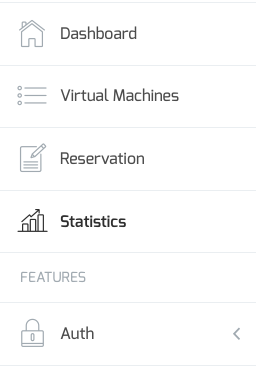
\includegraphics[height=0.4 \textheight]{menu}}
    \caption{Menu aplikacji}
  \end{figure}

  Ponadto u góry okna znajdziemy przycisk (
\includegraphics[height=1 em]{button_menu}) zmniejszający część okna zajmowaną przez menu, przełącznik \textbf{Light/Cosmic} pozwalający zmienić styl interfejsu, oraz przycisk (
\includegraphics[height=1 em]{button_layouts}) pozwalający między innymi przenieść menu na prawą stronę okna.

  \section{Virtual Machines}
  \label{VMs}

  \begin{figure}[H]
    \centerline{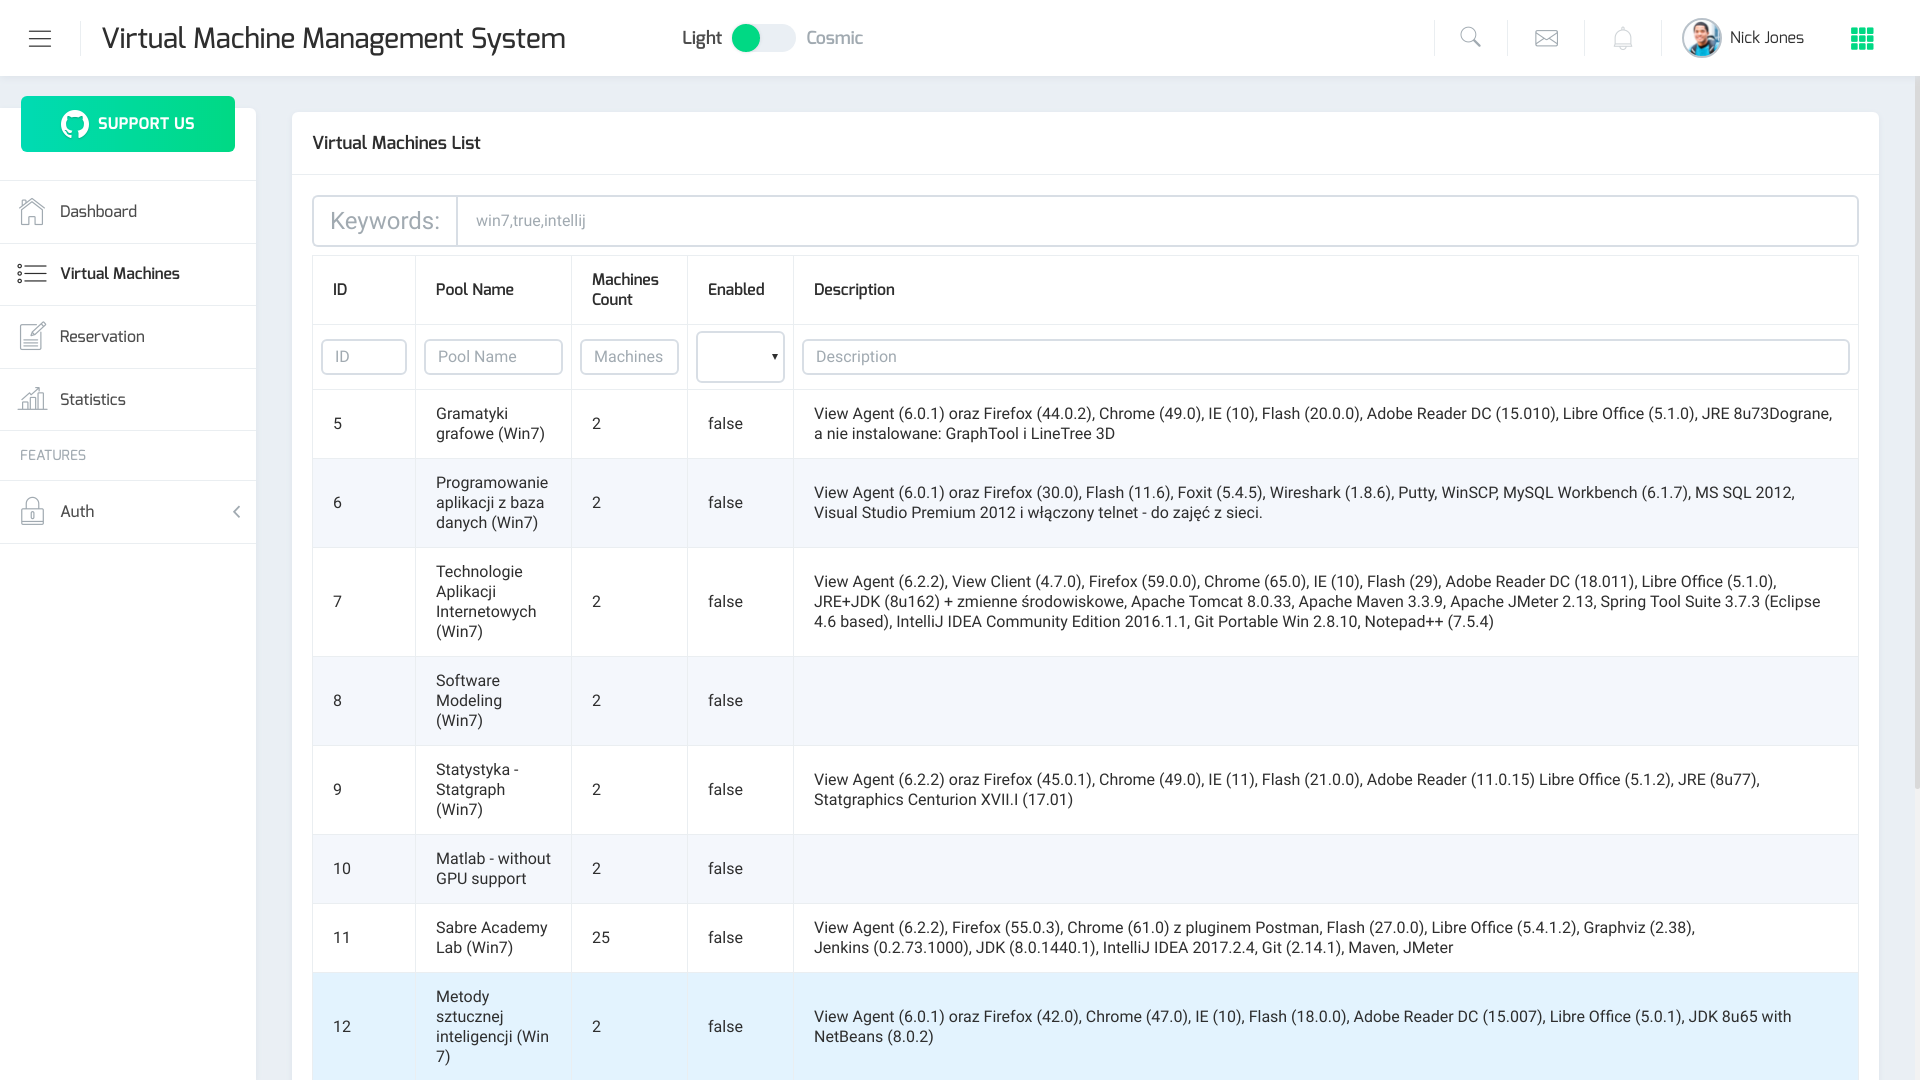
\includegraphics[width=0.9 \textwidth]{list}}
    \caption{Widok \textbf{Virtual Machines List}}
  \end{figure}

  Po wybraniu z~menu wpisu \textbf{Virtual Machines} zostaniemy przeniesieni do panelu \textbf{Virtual Machines List}. Jego główną częścią jest lista wszystkich dostępnych maszyn - tak włączonych, jak i~wyłączonych. Klikając na~poszczególne nazwy kolumn możemy włączyć sortowanie po wybranej kolumnie. Tuż pod nazwami kolumn znajdują się pola tekstowe umożliwiające ich filtrowanie -- wyświetlanie tylko rekordów zawierających w danej kolumnie wpisane słowo.

  Ponad listą maszyn znajduje się pole do~wyszukiwania po słowach kluczowych. Wpisane w~nie słowa lub liczby, oddzielone przecinkami, bez spacji, muszą wystąpić w~dowolnej kolejności w~dowolnej kolumnie wpisu, aby został on wyświetlony.

  \section{Reservations}

  \begin{figure}[H]
    \centerline{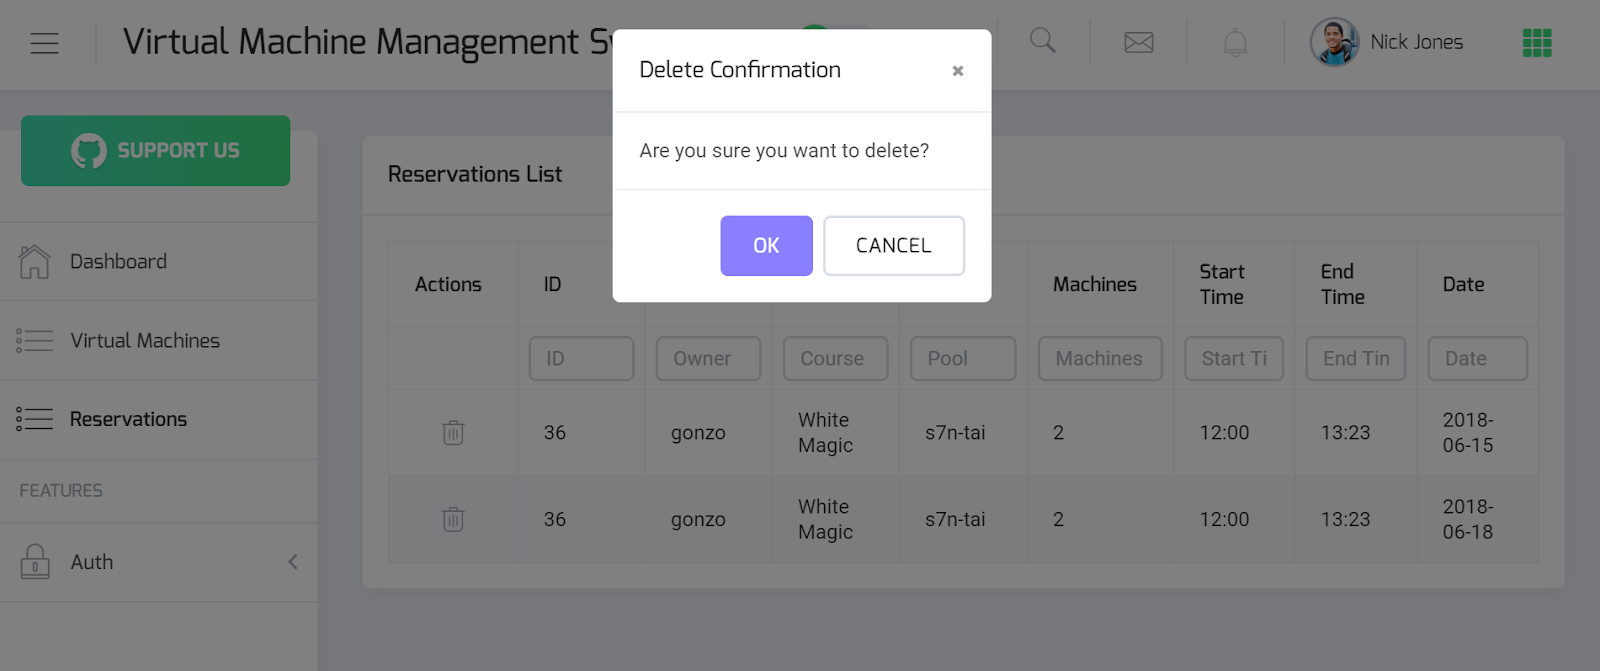
\includegraphics[width=0.9 \textwidth]{removing}}
    \caption{Widok \textbf{Reservations List}}

    Wybranie z menu opcji \textbf{Reservations} skutkuje przeniesieniem do widoku \textbf{Reservations List}. Lista umożliwia filtrowanie po zawartości kolumn i sortowanie po każdej z kolumn.

    W tym widoku można też usuwać poszczególne terminy rezerwacji za pomocą ikony kosza dostępnej przy każdym rekordzie listy. Przed faktycznym usunięciem program zapyta o potwierdzenie.
  \end{figure}

  \section{Reservation}

  \begin{figure}[H]
    \centerline{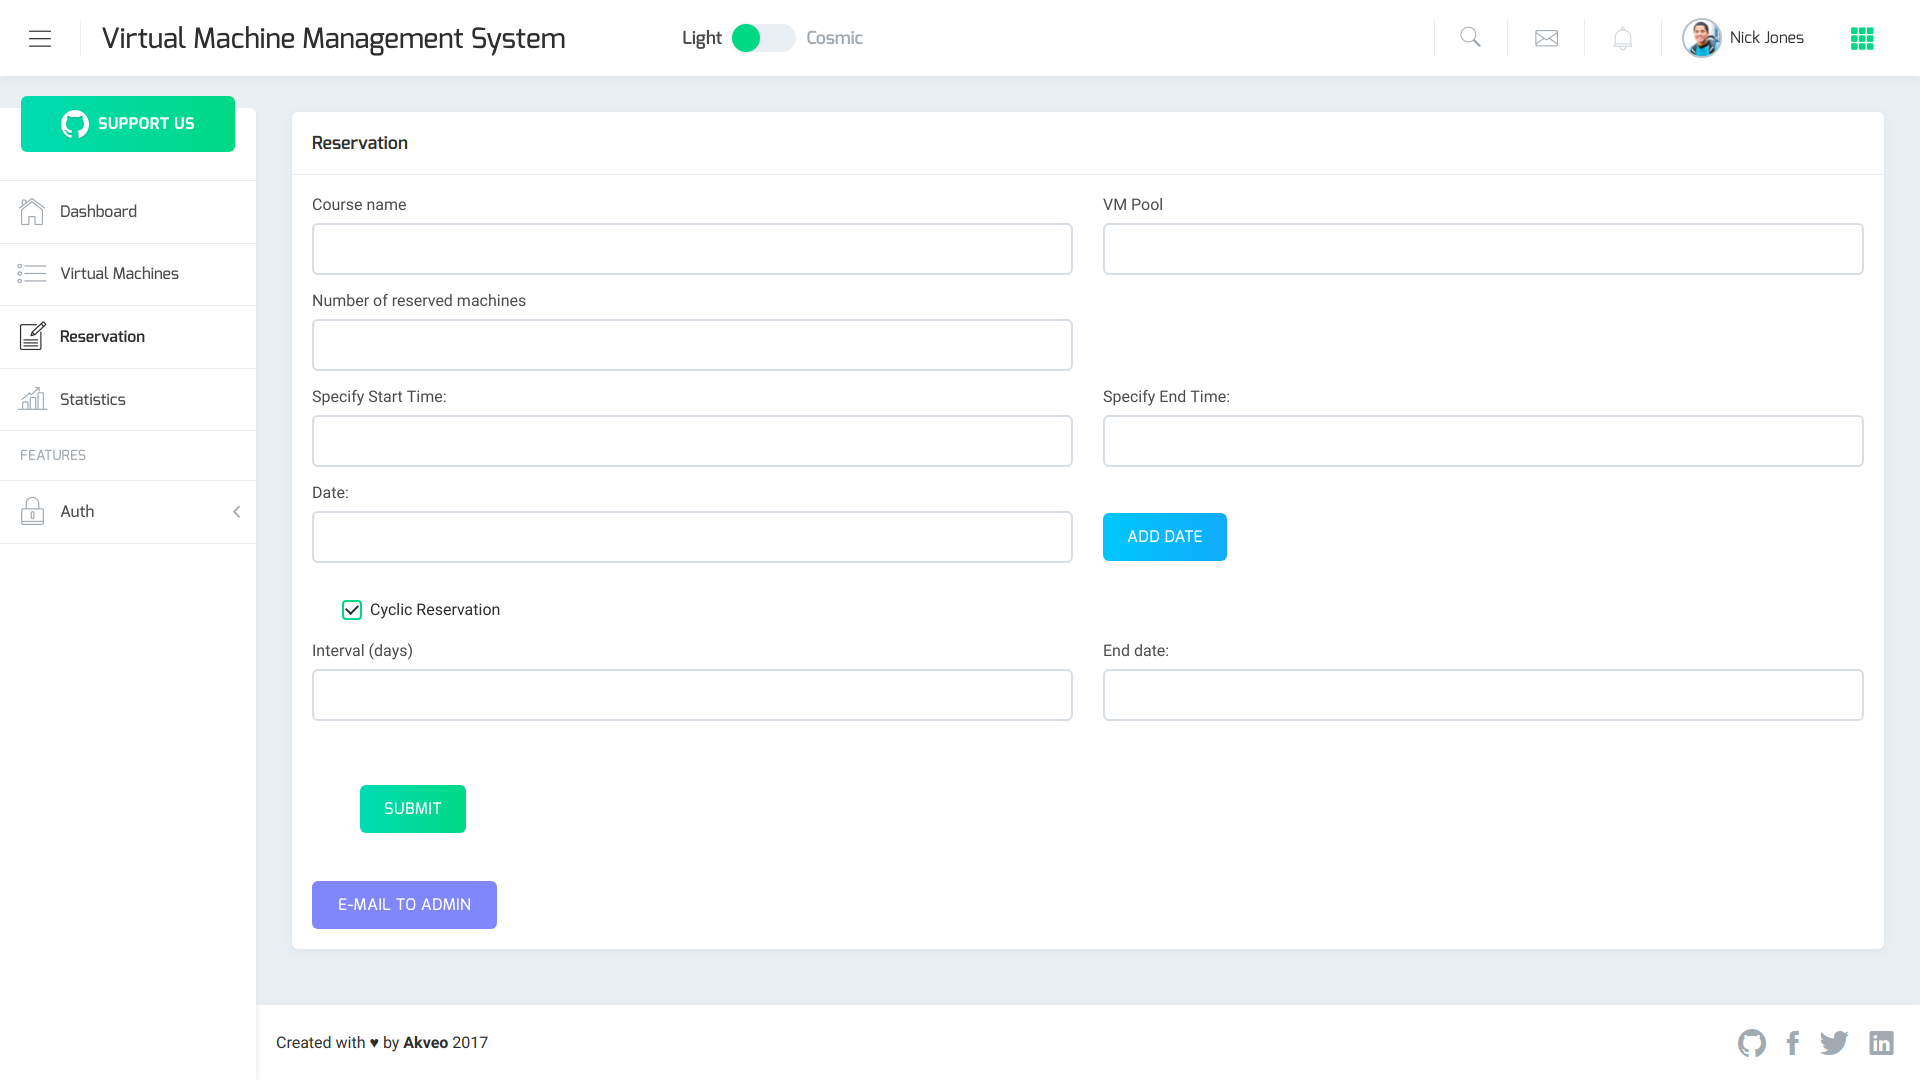
\includegraphics[width=0.9 \textwidth]{reservation}}
    \caption{Widok \textbf{Reservation}}
  \end{figure}

  Po wybraniu z~menu wpisu \textbf{Reservation} zostaniemy przeniesieni do panelu umożliwiającego utworzenie nowej rezerwacji. Wprowadzamy w~nim nazwę kursu, na potrzeby którego rezerwujemy maszyny, nazwę puli maszyn, z~której maszyny potrzebujemy (po rozpoczęciu wpisywania system podpowiada dostępne opcje), liczbę faktycznie wykorzystywanych maszyn oraz czas, kiedy ich potrzebujemy.

  Nazwa kursu jest nazwą definiowaną przez użytkownika i~jest stosowana w~celach identyfikacyjnych (nie ma zbioru prawidłowych wartości).

  Pule maszyn różnią się licznością, dostępnością i~zainstalowanym oprogramowaniem. Aby zapoznać się z parametrami pul, albo znaleźć taką, która odpowiada wymaganiom kursu, można użyć panelu \textbf{Virtual Machines} opisanego na stronie \pageref{VMs}.

  Na tym ekranie wpisujmy liczbę maszyn, których faktycznie zamierzamy używać. Dzięki temu kilka osób może równolegle korzystać z tej samej puli. Liczba ta oczywiście nie może być większa niż liczba maszyn dostępnych ogółem w~wybranej puli. W przypadku, gdy liczba maszyn w puli jest niewystarczająca, lub w~ogóle nie~ma puli odpowiadającej potrzebom, możemy wykorzystać przycisk \textbf{EMAIL TO ADMIN} opisany poniżej, aby zgłosić problem administracji.

  Po wpisaniu godziny rozpoczęcia zajęć w~polu \textit{Specify Start Time} pole \textit{Specify End Time} zostanie automatycznie wypełnione czasem zakończenia półtorej godziny późniejszym. Wartość tą można modyfikować. W~polu poniżej wybieramy datę, w~której ma obowiązywać nasza rezerwacja, a~klikając przycisk obok, możemy dopisywać kolejne daty. Niżej dostępne jest również pole wyboru \textit{Cyclic Reservation}. Po jego wybraniu możemy wskazać co ile dni ma być powtarzana nasza rezerwacja, i~od jakiego terminu już maszyny nie~potrzebujemy.

  \begin{framed}\textbf{Przykład:} potrzebujemy maszyn od przyszłego tygodnia do końca semestru, w każdy poniedziałek i środę, od godziny 10:00 do 13:30.
  
  Wpisujemy wówczas czas początkowy 10:00, czas końca 13:30, wybieramy datę najbliższego poniedziałku, kilkamy \textbf{ADD DATE}, w~nowym polu wybieramy datę najbliższej środy, zaznaczamy pole \textit{Cyclic Reservation}, wpisujemy interwał równy 7 dni, a~datę końca ustawiamy na~datę końca semestru.
  \end{framed}

  Gotową rezerwację zatwierdzamy przyciskiem \textbf{SUBMIT}. Jeżeli przynajmniej część żądanych maszyn nie jest dostępna, zostanie wyświetlony stosowny komunikat. Możemy w nim zdecydować, czy chcemy zarezerwować te maszyny, które są dostępne.

  \subsection{EMAIL TO ADMIN}

  \begin{figure}[H]
    \centerline{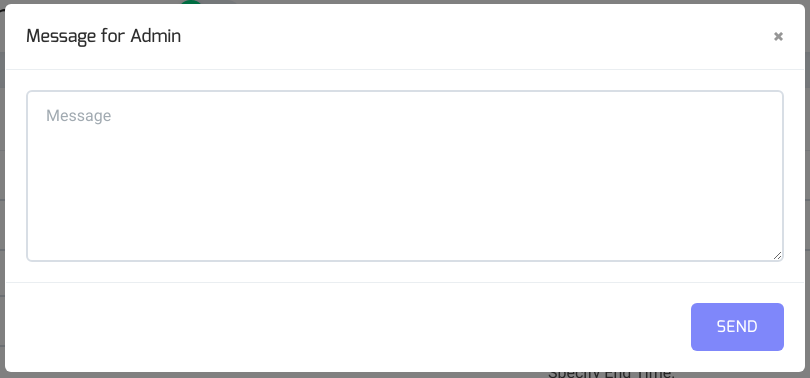
\includegraphics[width=0.9 \textwidth]{email}}
    \caption{Moduł wysyłania wiadomości e-mail}
  \end{figure}

  Przycisk \textbf{EMAIL TO ADMIN} pozwala na wysłanie wiadomości e-mail do~administratora maszyn wirtualnych. Po jego kliknięciu pojawia się prosty interfejs, w~którym w~polu tekstowym należy opisać swój problem lub prośbę. Po kliknięciu przycisku \textbf{SEND} e-mail jest wysyłany przez system, a~okno jest zamykane.

  \section{Statistics}

  \begin{figure}[H]
    \centerline{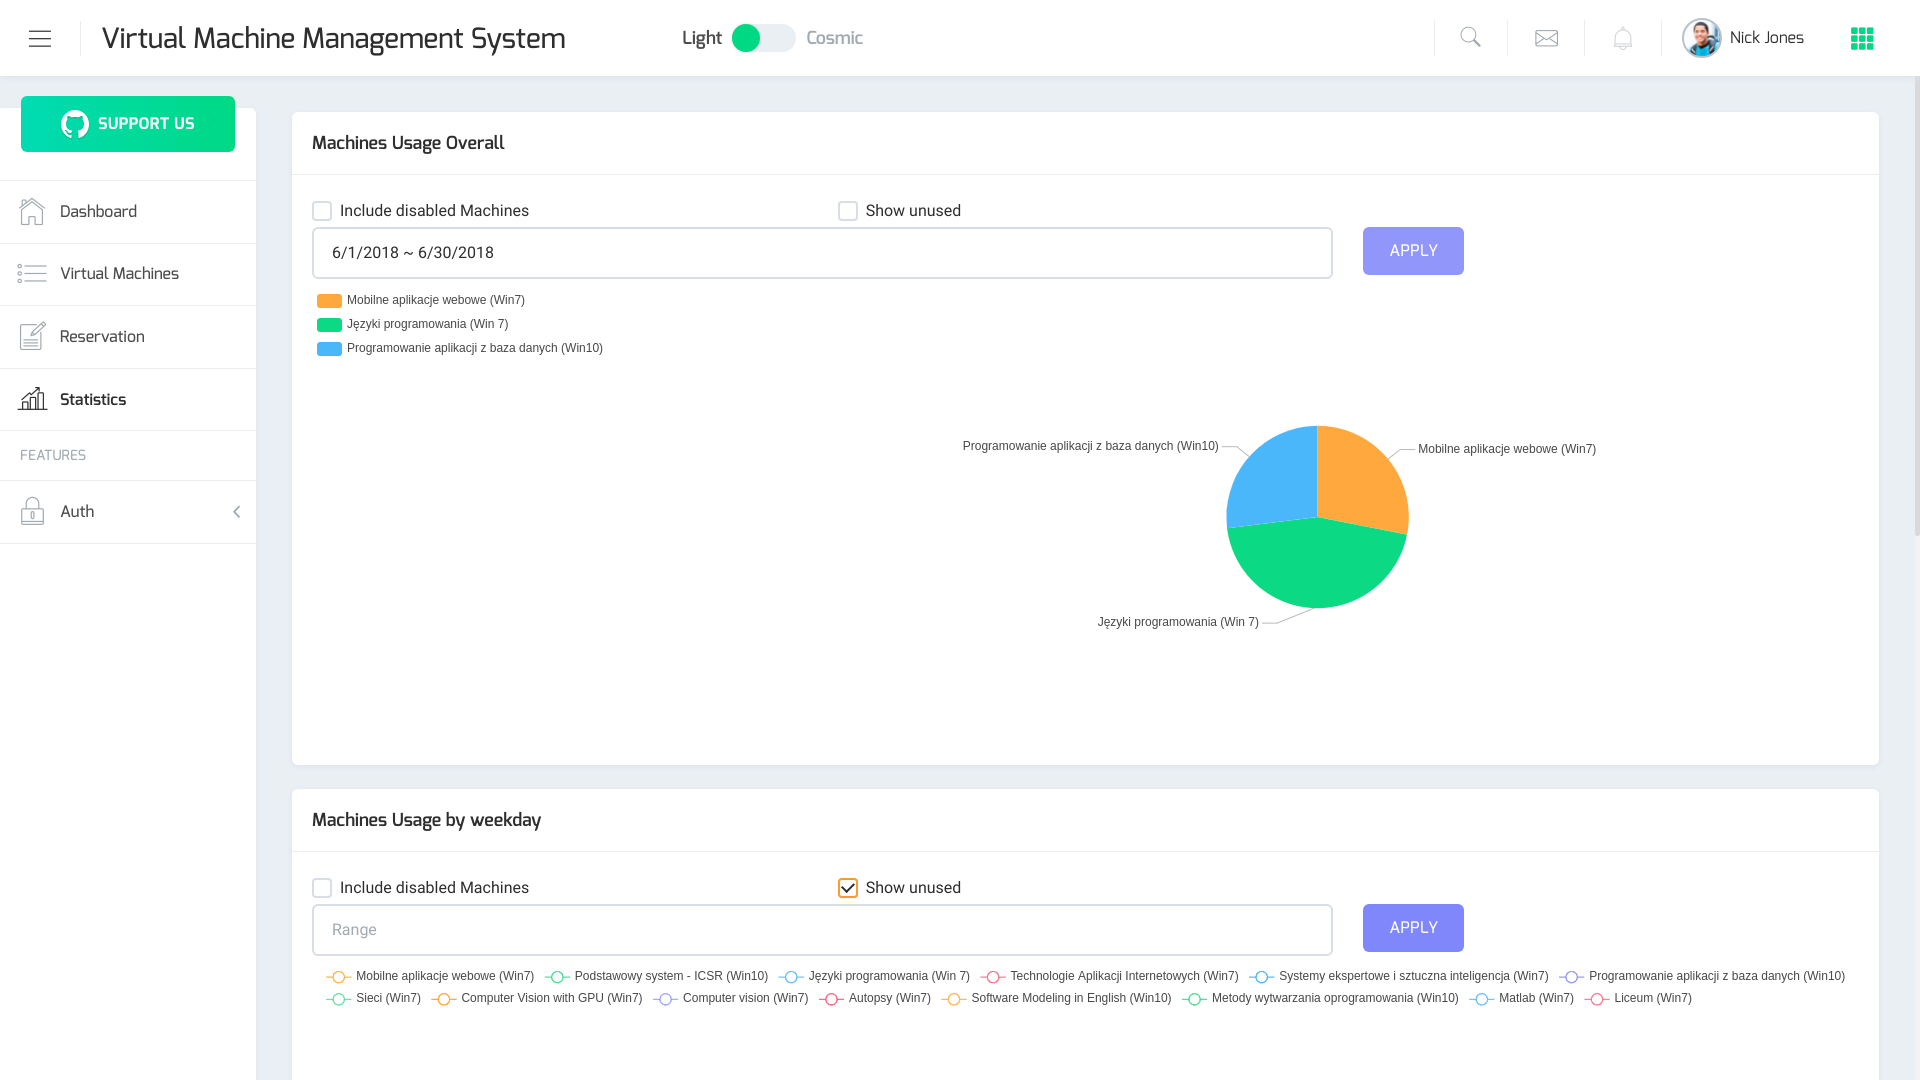
\includegraphics[width=0.9 \textwidth]{statistics}}
    \caption{Widok \textbf{Statistics}}
  \end{figure}

  Po wybraniu tej opcji w~menu, możemy zapoznać się z~szeregiem statystyk:

  \subsection{Machines Usage Overall}
  \label{MachinesUsageOverall}

  \begin{figure}[H]
    \centerline{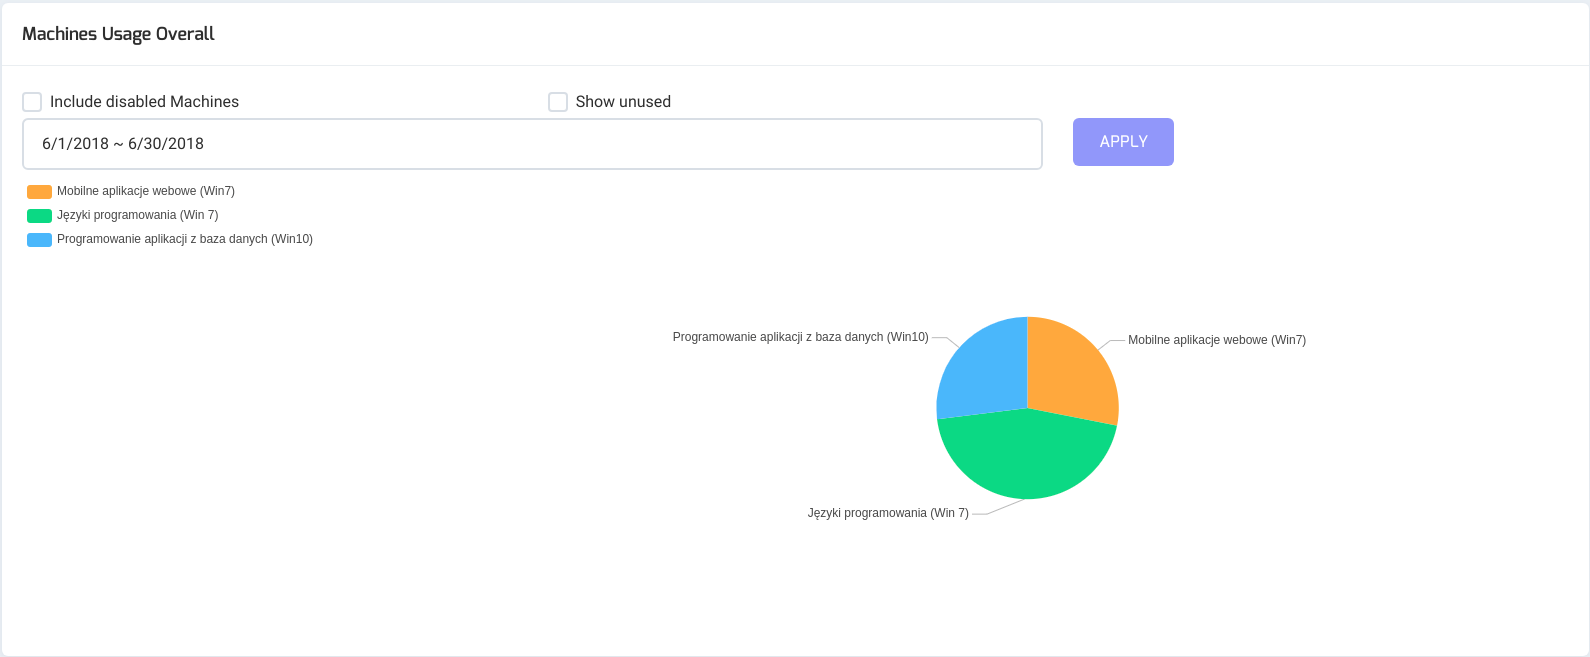
\includegraphics[width=0.9 \textwidth]{statistics_1}}
    \caption{Statystyka \textbf{Machines Usage Overall}}
  \end{figure}

  Wykres pokazuje liczbę maszynogodzin, na~jaką zostały zarezerwowane maszyny danej puli w~danym okresie.
  \begin{framed}
    \textbf{Przykład:} 5 maszyn, wypożyczonych na 4 godziny każda, to 20 maszynogodzin.
  \end{framed}

  W~polu \textbf{Range} należy podać interesujący nas przedział dat, którego ma dotyczyć statystyka -- zatwierdzamy wybór przyciskiem \textbf{APPLY}. Pola wyboru powyżej pozwalają zdecydować, czy chcemy wyświetlać nieaktywne pule maszyn, oraz czy interesują nas pule maszyn w~ogóle nie wykorzystywane w zadanym okresie -- te wybory również zatwierdzamy przyciskiem \textbf{APPLY}.

  Obok właściwego wykresu znajduje się legenda. Najeżdżając kursorem na~poszczególne wpisy wyróżniamy wartość na~wykresie, natomiast kliknięciami na~wpis powodujemy jego ukrycie lub pokazanie.

  \subsection{Machines Usage by weekday}
  \label{MachinesUsageByWeekday}

  \begin{figure}[H]
    \centerline{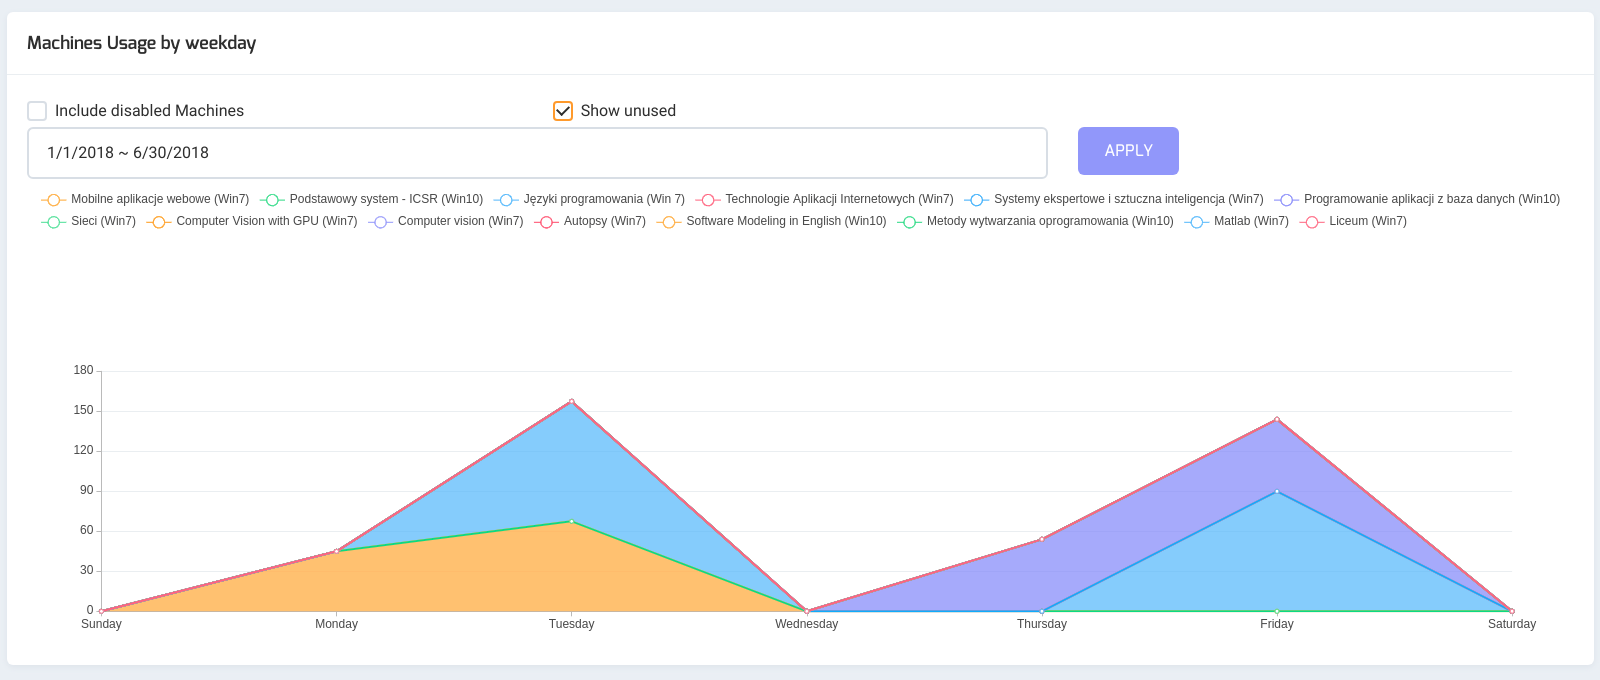
\includegraphics[width=0.9 \textwidth]{statistics_2}}
    \caption{Statystyka \textbf{Machines Usage by weekday}}
  \end{figure}

  Wykres pokazuje dynamikę wykorzystania pul maszyn w ciągu tygodnia. Wartości wyrażane są w~maszynogodzinach, jak zostały zdefiniowane w~sekcji \ref{MachinesUsageOverall}, dokładnie tak samo jak w~niej wybieramy także okres, oraz czy interesują nas maszyny nieaktywne lub nieużywane. Ponownie odznaczając wpisy w legendzie możemy ograniczyć liczbę pul uwzględnionych na~wykresie.

  Statystykę można wykorzystać do rozpoznania maszyn wykorzystywanych tylko podczas zajęć odbywających się~w~określonym dniu tygodnia; być może istnieje w~systemie inna pula o~tych samych właściwościach, wykorzystywana w~inne dni?

  \subsection{Monthly Usage}

  \begin{figure}[H]
    \centerline{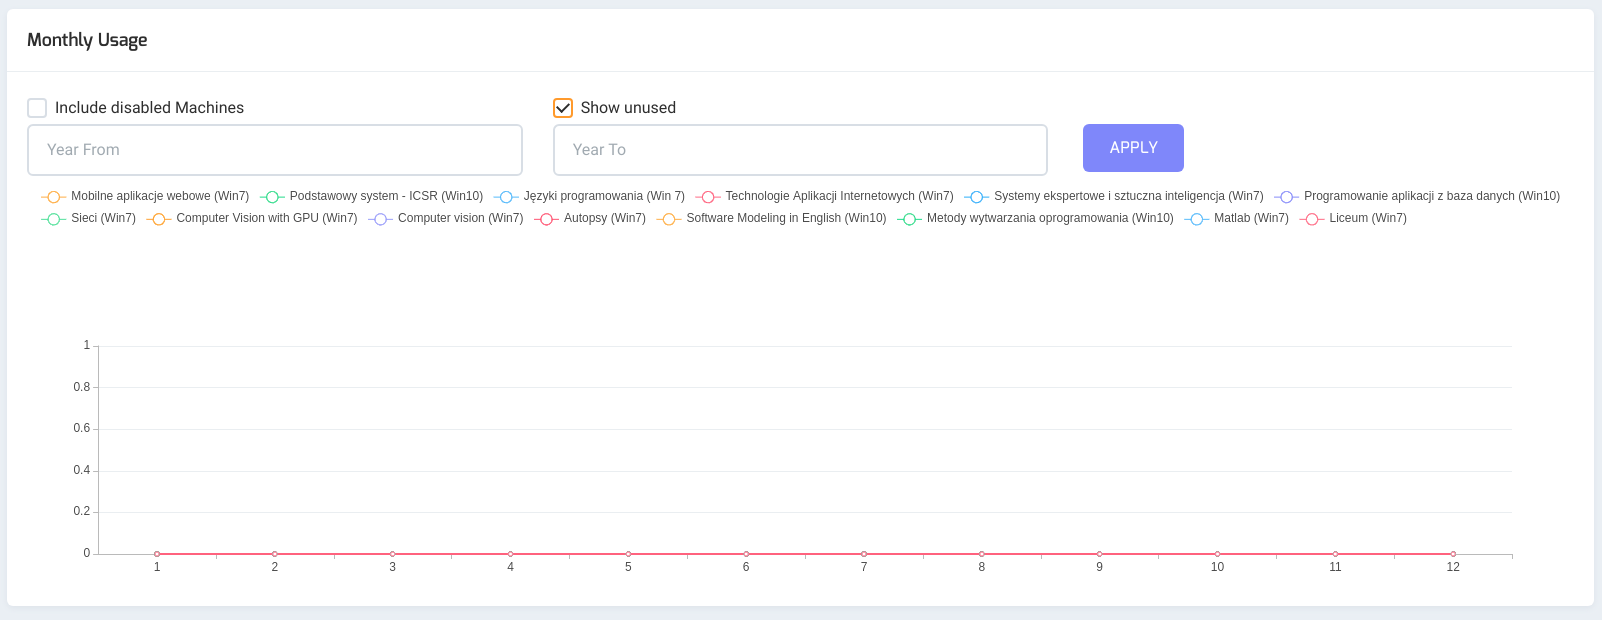
\includegraphics[width=0.9 \textwidth]{statistics_3}}
    \caption{Statystyka \textbf{Monthly Usage}}
  \end{figure}

  Statystyka funkcjonuje analogicznie jak \textbf{Machines Usage by weekday} z~sekcji \ref{MachinesUsageByWeekday}. W~tym przypadku jednak, możemy zaobserwować użycie maszyn w poszczególnych miesiącach. Jest to szczególnie przydatne do określenia, czy pewne pule wykorzystywane są tylko w jednym z~semestrów.

\end{document}